

\subsection{Iskanje intervalov}
 Naj bodo oznake kot zgoraj. Naj bo
\begin{gather*}
d(t) = {\bf n}\cdot({\bf f}(t) - {\bf b}_0),\\
d_0(t)= {\bf n}\cdot ({\bf p}(t) - {\bf b}_0),\\
d_1(t) = {\bf n}\cdot ({\bf p}_1(t) - {\bf b}_0) = d_0(t) + \delta, \\
d_2(t) = {\bf n}\cdot ({\bf p}_2(t) - {\bf b}_0) = d_0(t) - \delta.
\end{gather*}
Potem velja ocena
$$
|d(t)-d_0(t)|=|{\bf n}\cdot({\bf f}(t)-{\bf p}(t))|\leq \lVert {\bf n}\rVert\cdot \lVert {\bf f}(t) - {\bf p}(t) \rVert \leq \lVert {\bf f}(t) - {\bf p}(t) \rVert _{\infty}^{[\alpha,\beta]} \leq \delta.
$$
To pomeni, da $d(t)$ leži v pasu med $d_1(t)$ in $d_2(t)$ kot prikazuje slika \ref{slika4}.
\begin{figure}[!h]
    \centering 
    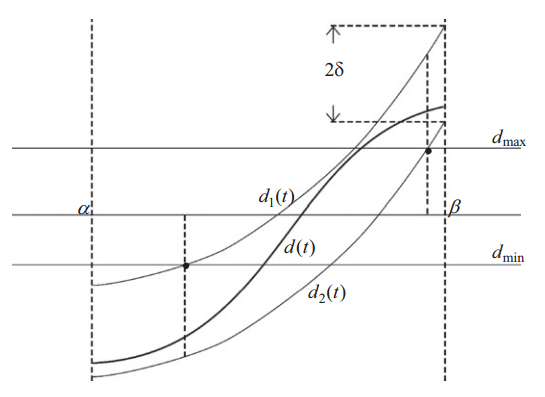
\includegraphics[width=0.6\textwidth]{dist}
    \caption{}
  	\label{slika4}
\end{figure}

Iz zgornjih dveh razdelkov vemo, da je predznačena razdalja točke ${\bf g}(t)$ od premice ${\bf b}_0{\bf b}_m$ vsebovana v intervalu $[d_{\text{min}}, d_{\text{max}}]$, in da je predznačena razdalja točke ${\bf f}(t)$ od premice ${\bf b}_0{\bf b}_m$ vsebovana v intervalu $[d_2(t), d_1(t)]$. Zato lahko tista območja, kjer je $d_1(t) < d_{\text{min}}$ in $d_2(t) > d_{\text{max}}$, zavržemo. Splošneje, če najdemo rešitve enačb
$$
d_1(t) = d_{\text{min}} \, \text{ in } \, d_2(t) = d_{\text{max}},
$$
potem lahko v domeni krivulje ${\bf f}$ najdemo iskane intervale $[\alpha _i, \beta _i]$, ki vsebujejo točke, ki se preslikajo v presečišča od ${\bf f}$ in ${\bf g}$.

V obeh zgoraj navedenih enačbah iščemo ničle polinoma. Če smo krivuljo ${\bf f}$ aproksimirali s krivuljo stopnje $2$ ali $3$, potem lahko ti dve enačbi rešimo analitično. To je v praksi najbolj učinkovita možnost.